\chapter{Màquines de vectors suport (Introducció als mètodes kernel)}
\section{Introducció}

Estem treballant amb models de la forma:
$$
y(x) = g(\boldsymbol{w}^T\boldsymbol{\phi}(x) + w_0),\ x \in \mathbb{R}^d, w \in \mathbb{R}^M, w_0 \in \mathbb{R}^d
$$
$$
\boldsymbol{\phi}(x) =
\begin{pmatrix}
\phi_1(x) \\
\phi_2(x) \\
\vdots \\
\phi_M(x)
\end{pmatrix}
$$

En xarxes neuronals es va dir que $\phi_i(x) = \phi(\varphi(x, v_i))$. 

Ara calculem un model lineal en l'espai de representació generat per les $\phi_i(x)$ (\textbf{feature space} = espai de característiques). El que fan els mètodes no lineals és buscar l'espai d'estadístiques adequat per a un problema en concret.

Una manera diferent de treballar és estudiar l'expressió:
\begin{align*}
	\phi(x)^T\phi(y) \quad x,y \in \mathbb{R}^d \\
	\phi: \text{feature map} 
\end{align*}

\textbf{Definim:} una funció de kernel $k: \mathbb{R}^d \times \mathbb{R}^d \rightarrow \mathbb{R}$ com:
$$
k(x,y) := \phi(x)^T\phi(y)
$$

\begin{itemize}
	\item Es poden estudiar les propietats de $k$ sense calcular (ni tan sols conèixer) $\phi$ de manera explícita.
	\item Es pot obtenir un algorisme d'aprenentatge \textbf{no lineal} partir d'un de lineal mitjançant l'ús de funcions de kernel (\emph{kernelitzar}).
	$$
	x^Ty \rightarrow \underbrace{\phi(x)^T\phi(y)}_{\mathclap{\text{$\phi$ no lineal, el resultat és un algorisme no lineal}}} = k(x,y)
	$$
\end{itemize}

\section{Com construir funcions de kernel}
Si tenim un 
$$
\phi(x) = 
\begin{pmatrix}
\phi_1(x)\\
\phi_2(x) \\
\vdots \\
\phi_n(x)
\end{pmatrix}
$$
$$
\implies k(x,y) = \phi^T(x)\phi(x) = \sum_{i=1}^M \phi_i(x)\phi_i(y)
$$

\textbf{Exemple} $(x^Ty)^3 \ ,x,y \in \mathbb{R}^3$
$$
x = \begin{pmatrix}
x_1 \\
x_2 \\
x_3
\end{pmatrix};
\quad 
y = \begin{pmatrix}
y_1 \\
y_2 \\
y_3
\end{pmatrix}
$$
\begin{align*}
	& (x^Ty)^3 = (x_1y_y + x_2y_2 + x_3y_3) = \\
	& (x_1y_1)^3 + 3(x_1y_1 + x_2y_2)^2 x_3y_3 + 3(x_1y_1 +
	 x_2y_2)(x_3y_3)^2 + (x_3y_3)^3 = ... \\
	& = 
	\begin{pmatrix}
	x_1^3 \\
	x_2^3 \\
	x_3^3 \\
	\sqrt{6} x_1x_2x_3 \\
	\sqrt{3} x_1^2x_2 \\
	\sqrt{3} x_1^2x_3 \\
	\sqrt{3} x_2^2x_1 \\
	\sqrt{3} x_2^2x_3 \\
	\sqrt{3} x_3^3x_1 \\
	\sqrt{3} x_3^3x_2 \\
	\end{pmatrix}^T 
	\begin{pmatrix}
	y_1^3 \\
	y_2^3 \\
	y_3^3 \\
	\sqrt{6} y_1y_2y_3 \\
	\sqrt{3} y_1^2y_2 \\
	\sqrt{3} y_1^2y_3 \\
	\sqrt{3} y_2^2y_1 \\
	\sqrt{3} y_2^2y_3 \\
	\sqrt{3} y_3^2y_1 \\
	\sqrt{3} y_3^2y_2
	\end{pmatrix}
	= \phi(x)^T\phi(y) \qquad \phi:\mathbb{R}^3 \rightarrow \mathbb{R}^{10}
\end{align*}

% FIGURA 2

$$
(x^Ty + 1)^3 \implies
$$
$\phi$ calcula tots els monomis de les variables (1,...,d) fins a grau 3. (0, 1, 2, 3).

$x^Ty$ \textbf{kernel lineal}

$\phi(x) = x$

$(x^Ty + 1)^2$ kernel quadràtic

$(x^Ty + 1)^3$ kernel cúbic

$(x^Ty + c)^q \quad ,c \ge 0, q \in \mathbb{N}$ kernel polinòmic

\textbf{Teorema} Una funció $k:\mathbb{R}^d \times \mathbb{R}^d \rightarrow \mathbb{R}$ és una \textbf{funció lineal} ($\exists \phi: \mathbb{R}^d \rightarrow \mathbb{R}^D, t.q. \ k(x,y) = \phi^T(x)\phi(y)$) si i només si:
\begin{itemize}
	\item $k$ és simètrica
	$$
		k(x,y) = k(y,x) \quad ,\forall x,y \in \mathbb{R}^d
	$$
	\item $\forall N \in \mathbb{N}$, per tota tria $x_1,...,x_N \ \mathbb{R}^d$, la matriu $K_{i,j} := k(x_i, x_j)$ és semi-definida positiva (PSD)
\end{itemize}

\textbf{Definició:} diem que una matriu $K_{N \times N}$ és PSD si és simètrica i $\forall c \in \mathbb{R}^N, c^T K c \ge 0$. És a dir $\sum_{i=1}^N\sum_{j=1}^N c_i K_{ij} c_j \ge 0$.

\textbf{Demostració:} Si la funció $k$ és un kernel $\implies K$ és PSD.
\begin{align*}
	& \sum_i \sum_j c_i K_{ij} c_j = 
	\sum_i \sum_j c_i \phi^T(x_i) \phi(x_j)c_j = \\
	& \left( \sum_i c_i \phi(x_i) \right)^T
	\left( \sum_j c_j \phi(x_j) \right) = 
	\left|\left| \sum_i c_i \phi(x_i) \right|\right|^2 \ge 0
\end{align*}

\textbf{Propietats}
Si $k$, kernels, $a \in \mathbb{R} \quad a \ge 0$:
\begin{itemize}
	\item $a·k$ kernel
	\item $k_1 + k_2$ kernel
	\item $k_1·k_2$ kernel
	\item p(k) kernel, si p és un polinomi de coeficients no negatius
\end{itemize}

\textbf{Proposició}
$$
k(x,y) = (x^Ty + c)^q \quad \forall c \ge 0, \forall q \in \mathbb{N}
$$

Podem definir funcions de kernel en qualsevol conjunt d'objectes o espai.
$$
k: \mathbb{R}^d \rightarrow \mathbb{R}^d 
\rightarrow \mathbb{R} \implies 
k: X \times X \rightarrow \mathbb{R}
$$
$X$ conjunt d'objectes finit (persones).

Una manera de comparar dos conjunts és comparar quants elements tenen en comú
$$
k(x,y) = | x \cap y|
$$
$$
x,y \subset X
$$
$$
I_X (M) = \begin{cases}
1 & \text{ si } M \in X \\
0 & \text{ si } M \cancel{\in} X
\end{cases}
$$
$$
|x \cap y| = \sum_{u \in X} I_X(u)·I_y(u) = k(x,y)
$$

\section{La dimensió VC per classificadors}
Es mesura la complexitat d'un model, per a un model lineal aquesta depèn del nombre de paràmetres. 

Sigui $\mathcal{F} = \{ y : \mathbb{R}^d \to \{ -1, +1 \} : y_0 \text{ està parametritzat per } \theta \in H \}$. Es fixen unes dades $\mathcal{D} = \{ (x_1, t_1),..., (x_N, t_N) \}$. Es diu que un classificador $y_0 \in \mathcal{F}$ trenca/esmicola (scatter) $\mathcal{D}$ si, per tota tria de les $t_n \ (1 \le n \le N)$ (hi ha $2^n$ tries diferents) $y_0$  classifica correctament les $x_n$.

\textbf{Definició} 

La dimensió VC de $\mathcal{F}$ és la $N$ més gran per la qual existeixen $x_1, ..., x_N \in \mathbb{R}$  tals que $\exists y_0 \in \mathcal{F}$ que les trenca (per a qualsevol configuració). 

\textbf{Exemple}

$$
\mathcal{F}_{lin}^d = \{ y(\boldsymbol{x}, \boldsymbol{w}) = signe(\boldsymbol{w}^T \boldsymbol{x} + w_0), 
\ \boldsymbol{x} \in \mathbb{R}^d, \ \boldsymbol{w} \in \mathbb{R}^d, \ w \in \mathbb{R}  \}
$$

\textbf{Proposició}: $\dim (\mathcal{F}_{lin}^d) = d + 1$.

\section{Màquines de Vectors Suport}

\begin{figure}[H]
	\centering
		
	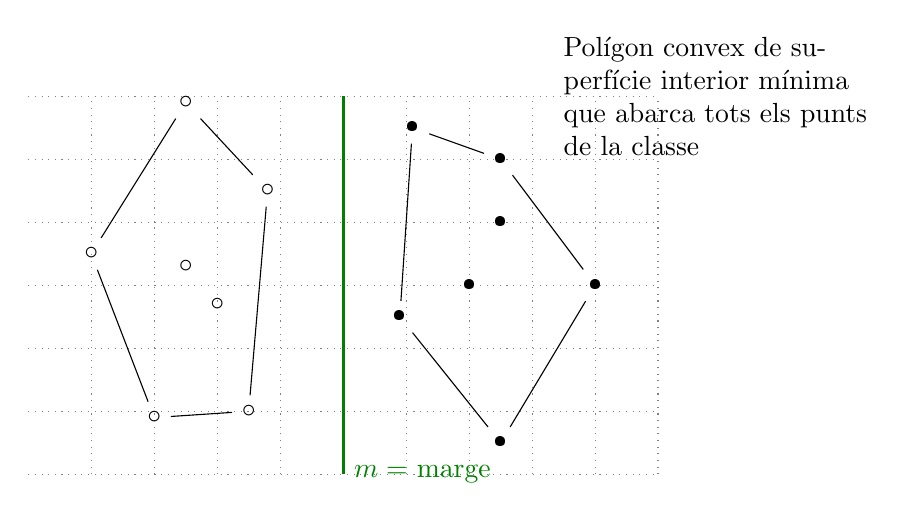
\begin{tikzpicture}[scale=8]
		\draw [step=0.1, dotted, gray] (-0.5,0) grid (0.5,0.6);
	
		\foreach \Point [count=\x] in {(0.09, 0.25), (0.25, 0.05), (0.4, 0.3), (0.25, 0.5), (0.11, 0.55), (0.2, 0.3), (0.25, 0.4)}{
			\node (right-\x) at \Point {\textbullet};
		}
		\foreach \Point [count=\x] in {(-0.15, 0.1), (-0.3, 0.09), (-0.4, 0.35), (-0.25, 0.59), (-0.12, 0.45), (-0.2, 0.27), (-0.25, 0.33)} {
			\node (left-\x) at \Point {$\circ$};
		}
	
		\foreach \x [remember=\x as \lastx (initially 1)] in{2,...,5,1}{
			\draw (right-\x) -- (right-\lastx);
			\draw (left-\x) -- (left-\lastx);
		}
	
		\draw[very thick, Green] (0,0) -- (0, 0.6) node[at start, right] {\textcolor{Green}{$m = $ marge}};
		
		\node[text width = 4cm] at (0.6, 0.6) {Polígon convex de superfície interior mínima que abarca tots els punts de la classe};
	\end{tikzpicture}
\end{figure}

Si es suposa que les dades són separables linealment. Es busca la recta que les separa deixant un marge $m$ màxim.

\begin{align*}
	\mathcal{D} &= \{ (x_1, t_1), ..., (x_N, t_N) \} \quad \text{S'assumeix $\mathcal{D}$ és separable linealment} \\
	& \phantom{{}={}}  
	\begin{aligned}
		\text{\textbf{def }} & y(x) = \op{sgn}(\boldsymbol{w}^T \boldsymbol{x} + w_0) \\
		& \text{on } \op{sgn}(z) = 
		\begin{cases}
			1 & \text{ si } z > 0 \\
			-1 & \text{ si } z < 0
		\end{cases}
	\end{aligned}
\end{align*}

\begin{align*}
	& \left[ \forall n : 1 \le n \le N : 
	\begin{rcases}
	\begin{cases}
		\bmath{w}^T x_n + w_0 > 0 & \text{ si } t_n = +1 \\
		\bmath{w}^T x_n + w_0 < 0 & \text{ si } t_n = -1
	\end{cases}
	\end{rcases} 
	\right] \\
	& \hspace{2em} \Updownarrow \\
	& \left[ \forall n : 1 \le n \le N : (\bmath{w}^T x_n + w_0) t_n > 0 \right]
\end{align*}

\textbf{Definició}: El \textbf{marge} d'un pla $\pi := $ distància de $\pi$ al punt més proper.

\textbf{Definició}: El \textbf{pla separador òptim} (PSO) $:=$ pla $\pi$ de màxim marge.

$$
\pi \left| \max_{\bmath{w}, w_0} \left( \min_{1 \le n \le N} d(x_n, \pi) \right)\right.
$$

Es normalitza $\bmath{w} \scalebox{1.8}{|} |\bmath{w}^T \bmath{x} + w_0| \ge 1$:

\textbf{Definició}: Els punts $x_n \scalebox{1.8}{|} |\bmath{w}^T \bmath{x} + w_0| = 1$ es diuen \textbf{vectors suport} (VS). 

\begin{itemize}
	\item El marge del PSO $\pi$ és: $d(x_{vs}, \pi) = 2 \frac{|\bmath{w}^T \bmath{x}_{vs} + w_0}{||w||} = \frac{2}{||w||}$
\end{itemize}

Així doncs el problema a resoldre s'escriu:

$$
\boxed{
\begin{aligned}
& \min_{\bmath{w},w_0} \frac{||w||^2}{2} \quad \text{Maximitzar el marge} \\
& \text{\textbf{subjecte a }} t_n (\bmath{w}^T x_n + w_0) \ge 1, \quad \forall n : 1 \ge n \ge N
\end{aligned}
}
$$

\textbf{Teorema} (Vapnik)

Es considera una classe de models $\mathcal{F}$ amb $\op{dimVC}(\mathcal{F}) = h$, amb probabilitat de com a mínim $1 - \eta$ on:

\begin{itemize}
	\item $E(y_D) \le E_D (y_D) + H(h, \eta, N)$ 
	\item $E(y_D)$ és l'error de generalització de $y_D$
	\item $E_D(y_D)$ és l'error de training de $y_D$ en les dades $\mathcal{D}$
	\item $y_D$ és un model de $\mathcal{F}$ obtingut amb les dades $\mathbb{D}$
	\item $H(h, \eta, N) = \left( \frac{h(\ln \frac{2N}{\eta} + 1) - \ln \frac{y}{4}}{N} \right)^{\frac{1}{2}}$ complexitat
\end{itemize}

\textbf{Teorema}

Sigui $\mathcal{F} = \{ y(x) = \op{sgn}(w^T x + w_0), \ w \in \mathbb{R}^d, \ w_0 \in \mathbb{R} \}$, considerem la subclasse $\mathcal{F}_n \subset \mathcal{F}$ que té marge $m \implies \dim VC(\mathcal{F}_m) \le \min \left( \left\lceil \frac{R^2}{m^2} \right\rceil, d \right) + 1$. On $R$ és el radi de l'esfera més petita que conté les dades. 

\subsection{Violacions del marge}

% Copiar d'Arnau, full 8-4

\begin{figure}[H]
	\centering
	\begin{tikzpicture}
		\begin{axis}[
				xmin=-0.1, xmax=1.1,
				ymin=-0.1, ymax=1.1,
				width=0.9\textwidth,
				height=0.9\textwidth
			]
			\addplot[blue, only marks] table [x=x, y=y]{tema_8/data/data1.csv};
			\addplot[red, only marks] table [x=x, y=y]{tema_8/data/data2.csv};
			\addplot[green, mark=none, very thick] {0.5};
			\addplot[green, mark=none] {0.55};
			\addplot[green, mark=none] {0.45};
			\addplot[purple, mark=none, very thick]{-x + 1};
			\addplot[purple, mark=none]{-x + 1.2};
			\addplot[purple, mark=none]{-x + 0.8};
			\draw[->] (axis cs:0.5,0.5) -- (axis cs:0.6,0.6) node[sloped, midway, above] {$m_2$};
			\draw[->] (axis cs:0.5,0.5) -- (axis cs:0.4,0.4) node[sloped, midway, above] {$m_2$};
			\draw[->] (axis cs:0, 0.5) -- (axis cs: 0, 0.55) node[midway, right] {$m_1$};
			\draw[->] (axis cs:0, 0.5) -- (axis cs: 0, 0.45) node[midway, right] {$m_1$};
			\draw[->] (axis cs:1, 0.5) -- (axis cs: 1, 0.55) node[midway, left] {$m_1$};
			\draw[->] (axis cs:1, 0.5) -- (axis cs: 1, 0.45) node[midway, left] {$m_1$};
		\end{axis}
	\end{tikzpicture}
\end{figure}


Si en lloc de separar les dades perfectament es tria un altre separador que cometi un cert error es pot aconseguir disminuir la dimensió VC del classificador. D'aquesta manera es pot violar el marge de separació per tal de disminuir la dimensió VC del classificador. \emph{Com s'escull aquesta violació? Quin nou marge s'escull? Com es quantifica la violació de marge?} El control del marge permet controlar el sobre-ajust també. 

\begin{itemize}
	\item Un cop es permeten aquestes violacions hi ha un compromís entre \emph{l'ajust de les dades} (separar tots els punts tant com sigui possible) i reduir \emph{la complexitat} (maximitzar el marge).
	
	\item S'introdueix un paràmetre de ponderació (\emph{cost parameter}): $C > 0$.
	
	$$
	\frac{min}{w_1 w_0 \textcolor{red}{,\varepsilon}} \frac{1}{2} ||w||^2 \textcolor{red}{+} \textcolor{Green}{C} \textcolor{red}{\cdot \sum_{n=1}^N \varepsilon_n}
	$$
	
	Subjecte a $t_n (w^T x_n + w_0) \ge 1; \quad (1 \le n \le N); \quad \textcolor{red}{\varepsilon_n \ge 0}$
	
	\begin{align*}
		& \textcolor{Green}{C \to \infty} & \textcolor{Green}{m \downarrow} & 
		\textcolor{Green}{\text{ sobreajust}} & \textcolor{Green}{\text{(separador 1)}} &
		\textcolor{Green}{\text{ errors de training } \downarrow} \\
		& \textcolor{red}{C \to 0} & \textcolor{red}{m \uparrow} & 
		\textcolor{red}{\text{ infrajust}} & \textcolor{red}{\text{(separador 2)}} &
		\textcolor{red}{\text{ errors de training } \uparrow}
	\end{align*}
\end{itemize}

\begin{align*}
	\mathcal{L} =& \frac{1}{2} ||w||^2  + C \cdot \sum_{n=1}^N \varepsilon - 
	\underbrace{\sum_{n=1}^N \mu_n \varepsilon_n}_{
		\mathclap{\text{\parbox{2cm}{restriccions \\ $\varepsilon_n \ge 0$}}}} 
	-\underbrace{\sum_{n=1}^N \alpha_n \{ t_n (w^T x_n + w_0) - 1 + \varepsilon_n \}}_{\mathclap{
		\text{\parbox{4cm}{restriccions \\ 
				$t_n (\bmath{w}^T \bmath{x_n} + w_0) + \varepsilon_n + 1 \implies$ \\
				$-t_n (\bmath{w}^T \bmath{x_n} + w_0) - \varepsilon_n + 1 \le 0 $ }}
	}} 
	\\
	& \alpha_n \ge 0 \\
	& \mu_n \ge 0
\end{align*}

\begin{align*}
	& \textbullet \frac{\partial \mathcal{L}}{\partial w_0} = - \sum_{n=1}^N \alpha_n t_n = 0 \implies \boxed{\sum_{n=1}^N \alpha_n t_n = 0} \\
	& \textbullet \frac{\partial \mathcal{L}}{\partial w} = w - \sum_{n=1}^N \alpha_n t_n x_n = 0 \implies \boxed{w = \sum_{n=1}^N \alpha_n t_n x_n} \\
	& \textbullet \frac{\partial \mathcal{L}}{\partial \epsilon_n} = C - \alpha_n - \mu_n = 0  \implies \boxed{C= \alpha_n + \mu_n}
\end{align*}
	
Substituim en $\mathcal{L}$ i obtenim el lagrangià dual $\mathcal{L}_{dual}$:

$$
\boxed{
\begin{aligned}
	&\mathcal{L}_{dual} = \sum_{n=1}^N \alpha_n - 
	\frac{1}{2} \sum_{n=1}^N \sum_{m=1}^N \alpha_n \alpha_m t_n t_m \textcolor{red}{x_n^T x_m} \\
	&\text{Subjecte a } 0 \le \alpha_n \le C
\end{aligned}
}
$$

\textcolor{red}{Kernelització! Substituïm $x_n$ per $\phi (x_n) \implies \phi(x_n)^T \phi(x_m) = K(x_n, x_m)$.}


\section{Kernelització de la SVM}

\begin{align*}
	& \min_{w, w_0, \varepsilon} \frac{1}{2} ||w||^2 + C \sum_{n=1}^N \varepsilon_n \\
	& \text{Subjecte a }
	\begin{rcases}
		& t_n (w^T \phi (x_n) + w_0) \ge 1 - \varepsilon_n \\
		& \phi: \mathbb{R}^d \to F \varepsilon_n \ge 0
	\end{rcases}
	1 \le n \le N
\end{align*}

\textbf{Lagrangià}
\begin{align*}
	& \mathcal{L} = \frac{1}{2} ||w||^2 + C \sum_{n=1}^N \varepsilon_n - 
	\sum_{n=1}^N \alpha_n \{ t_n (w^T \phi(x_n) + w_0) + \varepsilon_n - 1 \} -
	\sum_{n=1}^N \mu_n \varepsilon_n \\
	& \text{Subjecte a } \sum_{n=1}^N \alpha_n t_n = 0
\end{align*}

$\bmath{\mathcal{L}_{\text{DUAL}}}$
\begin{align*}
	&\max_{\alpha} \mathcal{L}_D = \sum_{n=1}^N \alpha_n - \frac{1}{2}
	\sum_{n=1}^N \sum_{m=1}^N \alpha_n \alpha_m t_n t_m \phi(x_n)^T \phi(x_m)\\
	& \text{Subjecte a } 0 \le \alpha_n \le C,\ 1 \le n \le C
\end{align*}

\begin{align*}
	y_{sum}(x) &= \op{sgn}(w^T \phi(x) + w_0) = 
	\op{sgn}\left( \left( \sum_{n=1}^N \alpha_n t_n \phi(x_n) \right)^T 
	\phi(x) + w_0 \right) = \\
	& \op{sgn} \left( \sum_{n=1}^N \alpha_n t_n \phi^T(x_n) \phi (x) + w_0 \right) = 
	\op{sgn} \left( \sum_{n=1}^N \alpha_n t_n \kappa(x_n, x) + w_0 \right) = \\
	& \op{sgn} \left( \sum_{n \in VS} \alpha_n t_n \kappa(x_n, x) + w_0 \right)
\end{align*}

\section{SVMs per regressió}

En regressió lineal clàssica regularitzada:

$$
\min_w \frac{1}{2} \sum_{n=1}^N (t_n - y(x_n))^2 + \frac{\lambda}{2}||w||^2
$$
$$
y(x_n) = w^T \phi(x_n)
$$

En SVMs, s'usa una funció que promou l'esparsitat:

\textbf{$\bmath{\varepsilon}$-insensibilitat:}

\begin{align*}
	\mathbb{E}_\varepsilon (y(x), t) = 
	\begin{cases}
		0 & \text{ si } | y(x) - t| < \varepsilon \\
		|y(x) - t| - \varepsilon & \text{ si } |y(x) - t| \ge \varepsilon
	\end{cases}
\end{align*}

\begin{figure}[H]
	\centering
	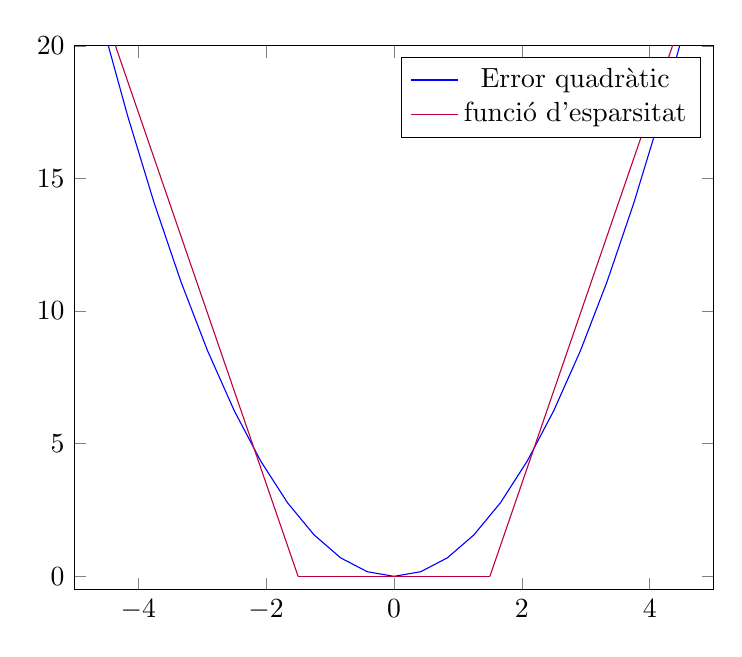
\begin{tikzpicture}
		\begin{axis}[
				xmin = -5, xmax = 5,
				ymin = -0.5, ymax = 20,
				width = 0.8\linewidth,
				height = 0.7\linewidth
			]
			\addplot+[mark=none] {x^2};
			\addplot+[mark=none, purple, domain=1.5:6] {7*x - 10.5};
			\addplot+[mark=none, purple, domain=-6:-1.5] {-7*x - 10.5};
			\addplot+[mark=none, purple, domain=-1.5:1.5]{0};
			\legend{Error quadràtic, funció d'esparsitat}
		\end{axis}
		% TODO S'hauria de posar -epsilon i +epsilon al grafic en lloc dels nombres
	\end{tikzpicture}
\end{figure}

S'introdueix dos jocs de variables: $\varepsilon_n$ i $\hat{\varepsilon}_n, \ 1 \le n \le N$.

\begin{itemize}
	\item $\varepsilon_n > 0 \ (\hat{\varepsilon}_n = 0)$, correspon a $t_n > y(x_n) + \varepsilon$. 
	\item $\hat{\varepsilon}_n > 0 (\varepsilon_n = 0)$, correspon a $t_n < y(x_n) - \varepsilon$.
	\item $t_n \in [ y(x_n) - \varepsilon, y(x_n) + \varepsilon]$. Es troba dins del marge.
	\begin{align*}
		& \implies \min_w \frac{1}{2}||w||^2 + C \sum_{n=1}^N (\varepsilon_n + \hat{\varepsilon}_n) \\
		& \text{Subjecte a } 
		\begin{rcases}
			& t_n \le y (x_n) + \varepsilon + \varepsilon_n \\
			& t_n \ge y(x_n) - \varepsilon - \hat{\varepsilon}_n \\
			& \varepsilon_n \ge 0 \\
			& \hat{\varepsilon}_n \ge 0
		\end{rcases} \\
		& \implies y_{SVM}(x) = \sum_{n \in VS} (\alpha_n - \hat{\alpha_n})\kappa(x_n, x) + w_0 \\
		& VS = \{ n | \varepsilon_n > 0 \text{ o } \hat{\varepsilon}_n > 0 \} \\
		& \varepsilon \to 0 \ \text{(SOBREAJUSTAT)} \\
		& \varepsilon \to \infty \ \text{(INFRAJUST)}
	\end{align*}
\end{itemize}
